\documentclass[tikz,border=6pt]{standalone}
\usepackage{amsmath,amssymb,mathtools,physics,bm,nicefrac,wasysym}
\usepackage{xcolor}

\definecolor{colone}{RGB}{180,60,60}
\definecolor{coltwo}{RGB}{60,110,180}
\definecolor{colthree}{RGB}{60,140,80}

\definecolor{accent}{HTML}{A13D2C}
\definecolor{accent2}{HTML}{2B5F6B}
\definecolor{muted}{HTML}{5A564F}
\definecolor{panel}{HTML}{F8F6F0}
\definecolor{linecol}{HTML}{D8D2C4}
\definecolor{ink}{HTML}{1E1C1A}
\definecolor{astroblue}{HTML}{1B4F72}
\definecolor{astrodark}{HTML}{17202A}
\definecolor{sunyellow}{HTML}{E8A33D}

\usetikzlibrary{calc,arrows.meta,positioning,decorations.pathreplacing,decorations.markings,angles,quotes,shapes.geometric}
\usepackage{tikz-3dplot}

\newcommand{\vecr}{\vec r}
\newcommand{\vecL}{\vec L}
\newcommand{\vecA}{\vec A}
\newcommand{\vecf}{\vec f}
\newcommand{\vecF}{\vec F}
\newcommand{\vecp}{\vec p}
\newcommand{\avg}[1]{\left\langle #1\right\rangle}
\newcommand{\vecx}{\vec x}
\newcommand{\hatn}{\hat n}
\newcommand{\rhat}{\hat r}
\newcommand{\phihat}{\hat\phi}
\newcommand{\thetahat}{\hat\theta}
\newcommand{\note}[1]{\textcolor{blue!60!black}{\textit{[#1]}}}

% Astronomical acronyms
\newcommand{\LST}{\mathrm{LST}}
\newcommand{\GST}{\mathrm{GST}}
\newcommand{\GMST}{\mathrm{GMST}}
\newcommand{\GAST}{\mathrm{GAST}}
\newcommand{\LMST}{\mathrm{LMST}}
\newcommand{\LAST}{\mathrm{LAST}}
\newcommand{\UT}{\mathrm{UT}}
\newcommand{\UTC}{\mathrm{UTC}}
\newcommand{\TAI}{\mathrm{TAI}}
\newcommand{\TT}{\mathrm{TT}}
\newcommand{\TDB}{\mathrm{TDB}}
\newcommand{\JD}{\mathrm{JD}}
\newcommand{\MJD}{\mathrm{MJD}}
\newcommand{\EoT}{\mathrm{EoT}}
\newcommand{\SNR}{\mathrm{SNR}}
\newcommand{\RON}{\mathrm{RON}}

% Helper commands for specific diagrams
\newcommand{\midlinelabel}[3]{
    \node (midlabel) at ($ (#1)!.5!(#2) $) {#3};
    \draw[stealth-] (#1) --  (midlabel);
    \draw[-stealth] (midlabel) -- (#2);
}
\newcommand{\midlinelabell}[3]{
    \node[fill = white, inner sep = 0.2pt, outer sep=3pt] (midlabel) at ($ (#1)!.5!(#2) $) {#3};
    \draw[stealth-] (#1) --  (midlabel);
    \draw[-stealth] (midlabel) -- (#2);
}
\newcommand{\midlinelabelll}[3]{
    \node[fill = white, inner sep = 0.2pt, outer sep=3pt,scale=0.6] (midlabel) at ($ (#1)!.5!(#2) $) {#3};
    \draw[stealth-] (#1) --  (midlabel);
    \draw[-stealth] (midlabel) -- (#2);
}



\begin{document}
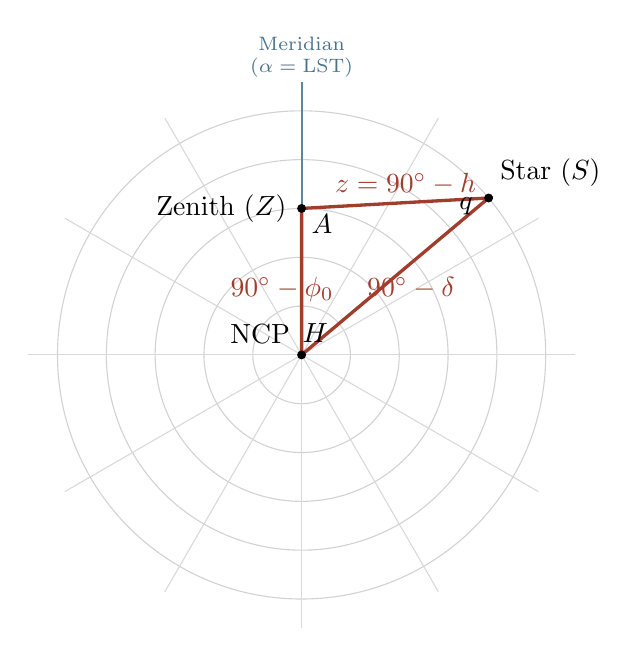
\begin{tikzpicture}[>=Stealth, scale=0.62, font=\scriptsize]
		\foreach \r in {1,2,3,4,5} {
			\draw[gray!35] (0,0) circle (\r);
		}
		\foreach \h in {0,2,...,22} {
			\draw[gray!30] (0,0) -- ({90+15*\h}:5.6);
		}
		\draw[astroblue!70, thick] (0,0) -- (0,5.6);
		\node[astroblue!80, font=\scriptsize, align=center] at (0,6.1) {Meridian\\($\alpha=\LST$)};

		\coordinate (NCPp) at (0,0);
		\coordinate (Zp) at (0,3);
		\coordinate (Sp) at ({5*cos(40)},{5*sin(40)});

		\draw[very thick, accent] (NCPp) -- (Zp) -- (Sp) -- cycle;

		\fill (NCPp) circle(2.6pt) node[above left=1pt, font=\normalsize] {NCP};
		\fill (Zp) circle(2.6pt) node[left=2pt, font=\normalsize] {Zenith ($Z$)};
		\fill (Sp) circle(2.6pt) node[above right=1pt, font=\normalsize] {Star ($S$)};

		\node[accent, font=\normalsize] at (-0.4,1.34) {$90^\circ-\phi_0$};
		\node[accent, font=\normalsize] at (2.24,1.37) {$90^\circ-\delta$};
		\node[accent, font=\normalsize] at (2.13,3.5) {$z=90^\circ-h$};

		\node[font=\normalsize] at (0.28,0.45) {$H$};
		\node[font=\normalsize] at (0.42,2.68) {$A$};
		\node[font=\normalsize] at (3.37,3.05) {$q$};
	\end{tikzpicture}
\end{document}
